\section{Design}
\label{sec-design}

\subsection{network design}

As mentioned above, we designed merging layers in our network so that we can process the input images by performing convolution operations to each single image, and then merging them together. The merged data will be stacked with the feature maps of each single image before we perform the next layer of convolution on them. Each convolutional layer uses the same set of parameters for all the images, so that the same set of features are extracted from the images, and thus can be merged. The merging layers consists of simple calculations extracting either the most significant, or the mutual features of the images, the former preserving interesting findings while the latter filters out credible features from the redundancy of the input. The network pipeline consists of alternate layers of convolution and merging, and after each merging layer, the reliable information accumulates and more complex features can be extracted with their support. Furthermore, we frequently insert the original input images in each level of our pipeline, creating an unevenness in depth and reducing network complexity, because we discovered that this process guides the model to be loyal to the inputs, generating more truthful results and less artifacts.

The details of our network architecture is as follows:
	Each input image (or each lane from the output of the previous layer) is assigned to its own lane and processed by several convolutional layers. These layers share parameters across channels; however, each image is processed individually and do not interact with each other in this stage. Each channel will present a feature map of n channels.
	The features extracted from all layers are merged broadwise with the following function:


    $${x'_k=\sum x_ie^{kx_i}/\sum e^{kx_i}}$$


Where k varies from -1 to 1. Apparently, k=0 leads to averaging, k=${+\infty}$ leads to a process similar to max operator and k=${-\infty}$ leads to min operator. This process merges information from every lane into one. The output is n channels for each value of k. 
	The original input images are accessed again. These images are also processed separately by several convolutional layers (sharing parameters across lanes) to extract features. The output of these images (m channels each) are stacked with the n channels from step 2) as m+n channels each lane. Some more convolution and an upscaling layer may follow, merging the data more thoroughly. These will be the input for the next layer.
The above 3 steps are stacked as one layer. The functional network often consists of 5 to 8 layers to achieve 4x super resolution. The network ends with a merging process similar to the 2) step and a few more layers of convolution. The full structure of a 3 layer network is shown in Fig~\ref{fig-system}.

\begin{figure}
 \centering
    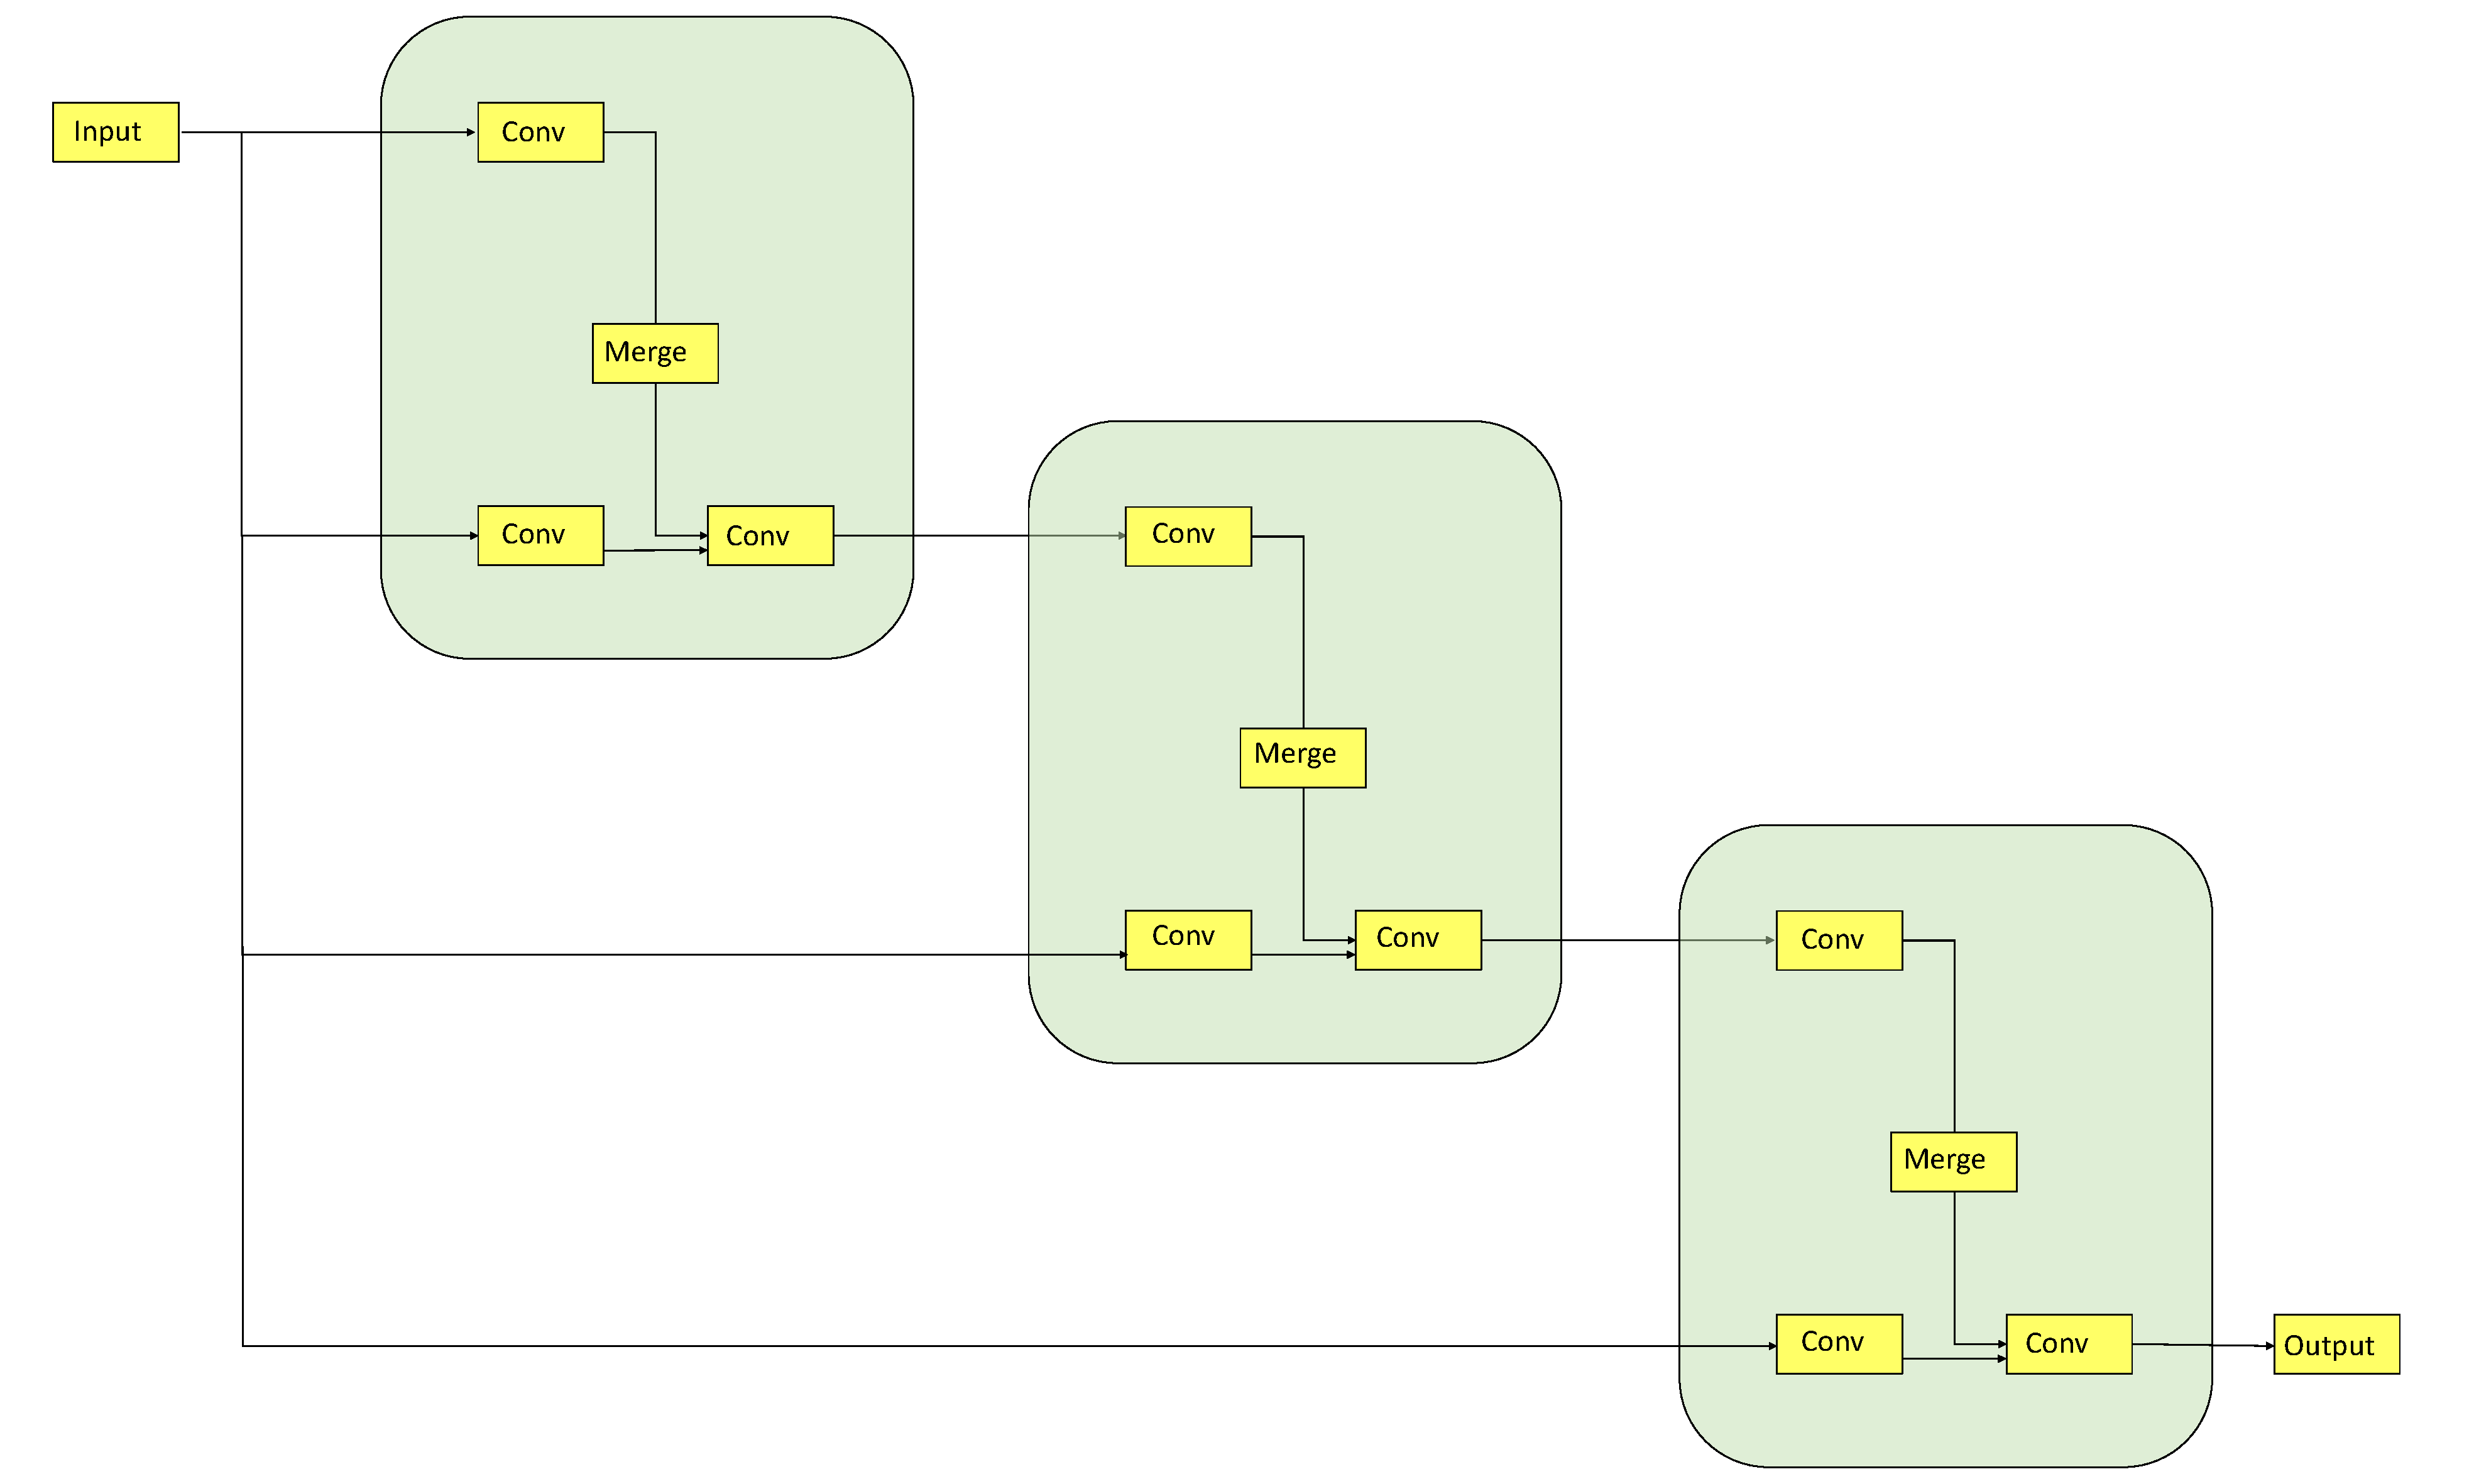
\includegraphics[width=0.5\textwidth]{./pic/design.pdf}
    \caption{Network Architecture of SRPeek.}
    \label{fig-system}
\end{figure}

\subsection{system design}


We implemented a holistic system for shoulder surfing, with the neural network as core, on a smartphone to verify the efficiency of our model. It iterates through the following steps: 
\begin{enumerate}

\item Input. Under guidance of the attacker, The smartphone will zoom in, take focus, and take 20 images with burst mode of the target screen. Note that the zoom in step is only for easier interaction and focusing, and to utilize the telephoto lenses and optical zoom, if avaliable, as digital zooming do not put in any extra data; On traditional phones with only digital zooming, the photo-taking will be with 1x zoom, and on phones with optical zooming, 5x to 10x zoom, depending on the optical zooming range. This way information on the images will be more compact and easier to comprehend by neural networks.

\item Alignment. The images are then aligned to mitigate the shifts between frames caused by hand tremor or movements from the lenses, as cameras with optical lenses will ocationally shift slightly across time due to the movements of its inner mechanism. Luckily, in our scenario the target is a glowing screen whose edges are easily distinguishable in most cases, and we use them as reference to align our images. The images are also spun to make the text horizontal in the process. The screen is cropped out and the rest of the image abandoned.

\item Adjustment. The lines of text(or stuff differing from the background color of the screen) will be carved out for processing, to reduce the workload of the network. The characters are normally around 10x10 pixels in the photos, and the carved segments will leave 2 pixels of padding on all sides to avoid mutilating the character; A certain amount of error is allowed, but if the size of the text is too small or too large, the neural network will not be able to extract features normally, so the images will be zoomed to the right size(and the zooming of step (1) will be adjusted accordingly).

\item Processing. As our network accepts only 9x9 patches, we will iteratively process all the overlapping 9x9 boxes among the input photo. For example, a 10x10 image will be four 9x9 patches, and a 11x11 image nine patches, etc(see fig.~\ref{fig-patches}. After carving a 9x9 patch at corresponding locations of each image, these patches are then processed by our multi-frame super resolution network, generating a single 36x36 image (4x upscaling). The input is RGB colored, while the output, as we are not interested in color, is black and white. When all patches are processed, their outputs are merged together. The overlapping pixels are thus processed: among all the outputs containing this pixel, we collect these values, remove outliers, and use their average as the result. In this way, we generate upscaled image segments of all the characters on the target screen, which are then inserted in one of the input images(roughly upscaled to encompass them, just for reference) and displayed to the attacker.

\begin{figure}
 \centering
    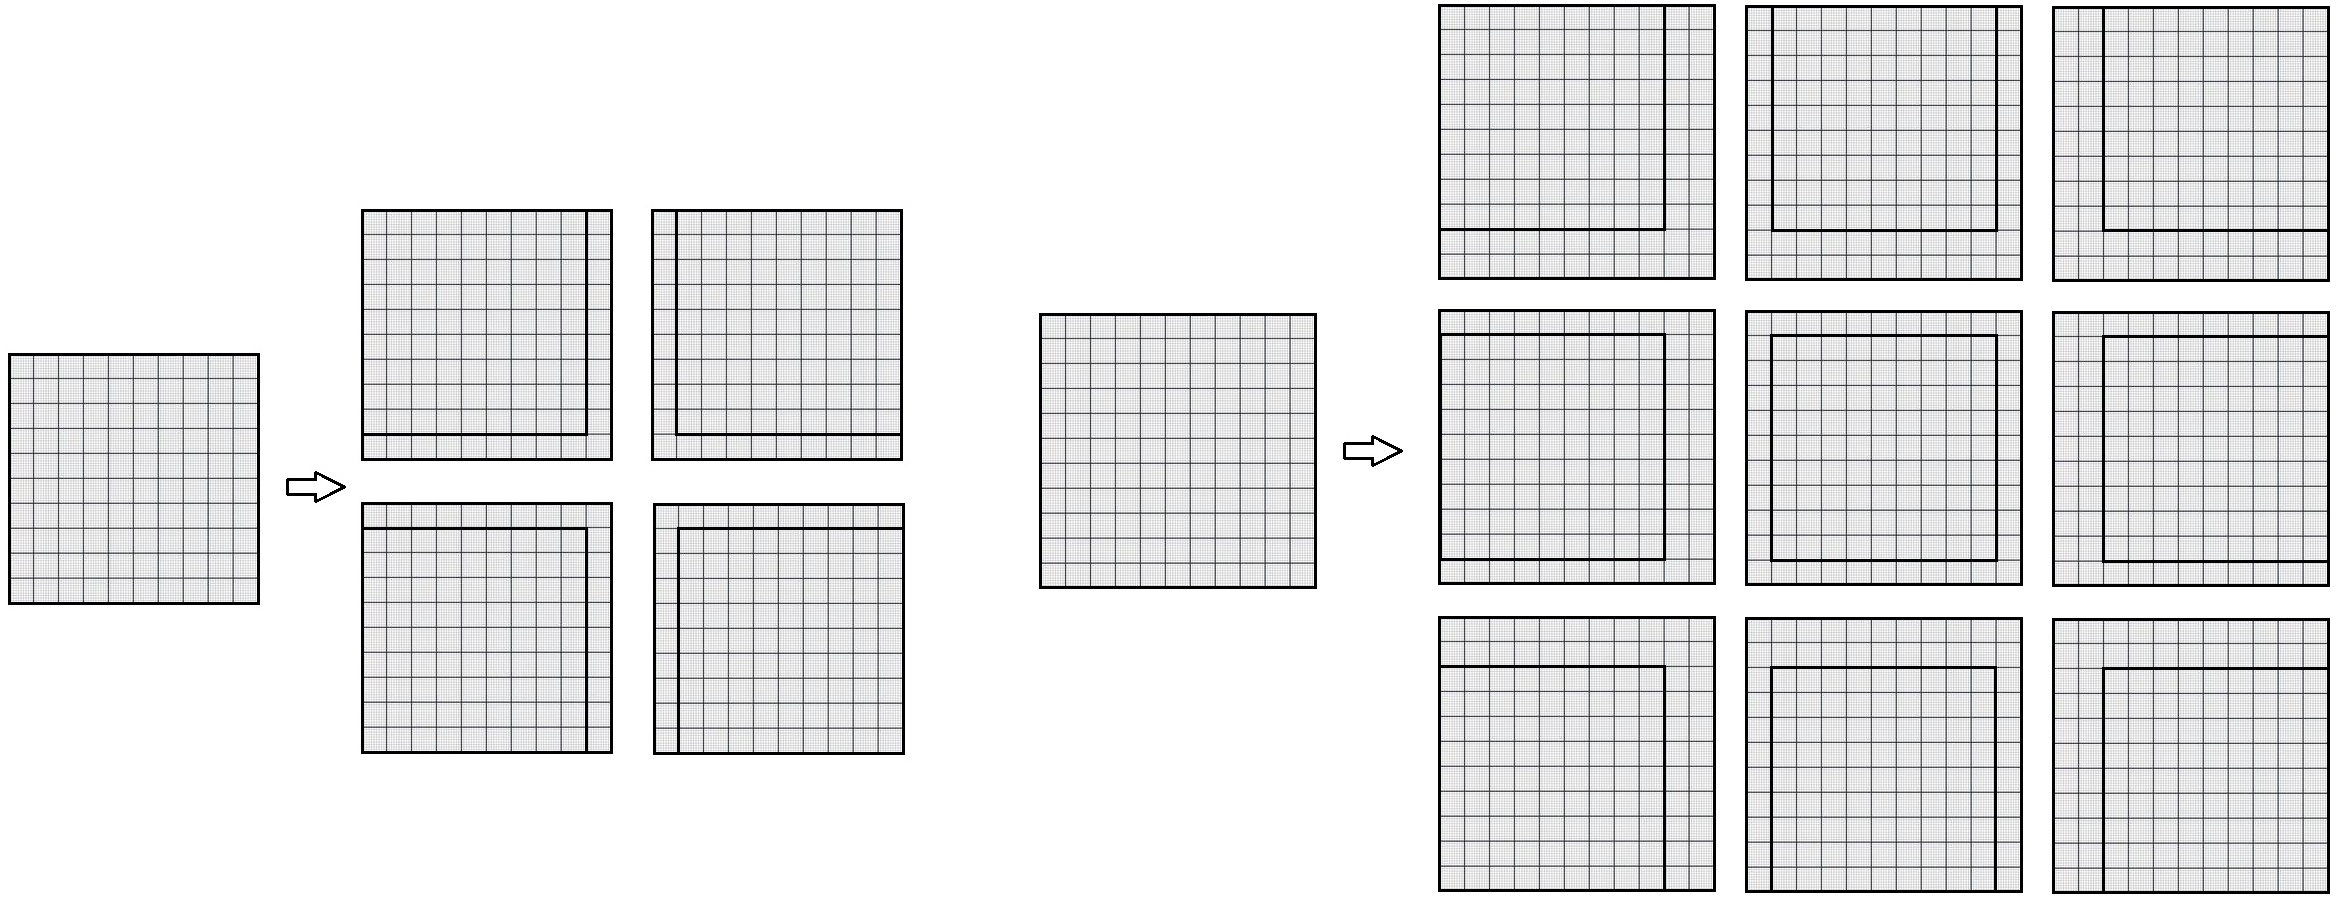
\includegraphics[width=0.5\textwidth]{./pic/patches.jpg}
    \caption{Illustration of overlapping patches the network process photos.}
    \label{fig-patches}
\end{figure}

\end{enumerate}

These steps are repeatedly executed to enable the attacker to monitor the victim. The workflow of our system is shown in fig.~\ref{fig-workflow}. The training data for the network is also gathered in this way. Different lenses have different photographing abilities and blurring patterns, so the model has to be trained for each phone with training images captured from it. When using smartphones with optical zoom, the images will shift slightly over time even if we keep them completely still, so the aligning phases are still needed. To reduce calculation and better align the images with the ground truth, we drew a box around the text on the victim's screen, replacing the edges of the phone for alignment and cropping in the alignment step (as shown in fig.~\ref{fig-workflow}), but our system works perfectly without it.
\begin{figure}
 \centering
    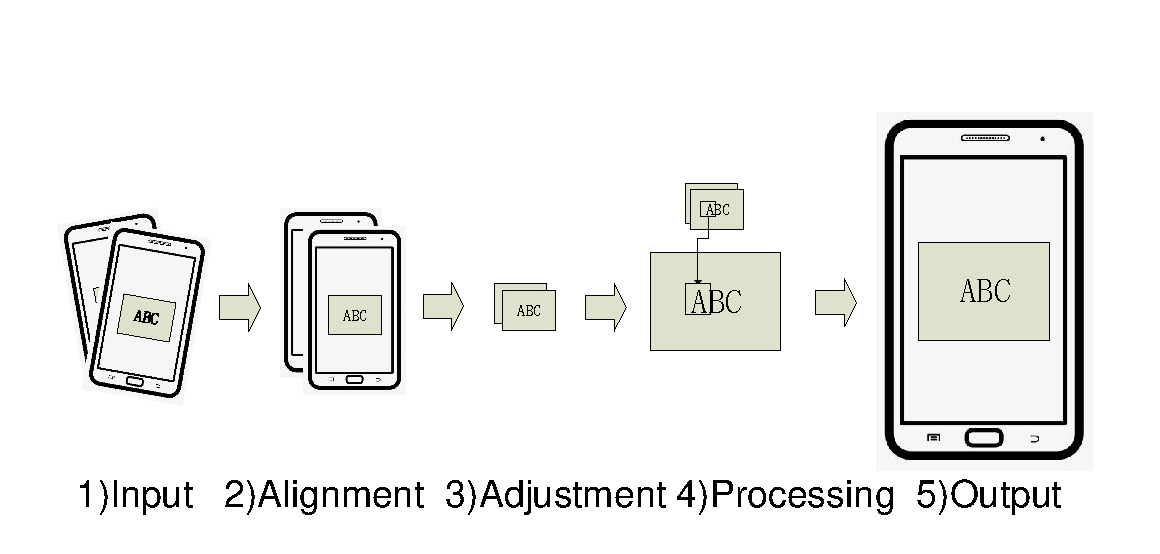
\includegraphics[width=0.5\textwidth]{./pic/workflow.pdf}
    \caption{Illustration of the workflow of our shoulder-surfing system.}
    \label{fig-workflow}
\end{figure}

